\chapter{绪论}
\section{研究背景与意义}
骨关节炎是一种由遗传因素与环境因素共同作用所产生的关节退行性病变,目前尚无有效的治疗方法。世界范围内至少三亿人罹患骨关节炎且患者群体逐年扩大。而其较差的预后也使得骨关节炎成为了全球范围内导致残疾与疼痛的主要因素之一。临床研究显示,早期诊断与介入对骨关节炎患者病程控制有着积极的影响。因此,构建骨关节炎患病风险预测模型有助于通过早期筛查与预警的方式帮助潜在患者控制病程发展。目前已有诸多关于骨关节炎基因型的全基因组关联研究(GWAS)鉴定了若干骨关节炎的易感SNP位点,也有相关研究基于这些位点建立了骨关节炎风险预测模型。但是这些模型的预测效果较差,远不能达到临床预测的要求。此外,现有的模型也无法处理输入基因型数据之间的复杂网络关系。同时这些模型只能根据输入的位点信息给出判断,无法解释输入位点之间的关联与特定位点在预测过程中的贡献值,模型可解释性方面存在较大不足。以上存在的问题与不足极大限制了骨关节炎风险预测模型的实际应用,如何改进构建模型的方法以提高模型的预测效果,也成为相关研究亟待解决的关键问题。

图作为一种数据结构能通过对节点与边的描述同时反映节点信息与节点之间关系,目前已被广泛应用于分子生物学代谢网络、动物行为学社交网络等生物学领域的研究中。鉴于基因型位点相互关联乃至成网的特征,同时考虑到图在提取和处理处理节点信息(特征)及节点间关系过程中的优势,本文使用图来描述基因型位点特征与位点-位点关系。但是,图数据作为一种非欧数据,传统的诸如卷积神经网络在内的机器学习方法并不适用于直接对图数据进行处理和分析。近年来随着图数据在各个领域的广泛应用,为了解决这一问题,适用于处理图数据的图神经网络因运而生。图神经网络能够基于图信息完成诸如图分类、节点分类等任务并且具有效果好、可解释性强等优点,适合用来处理基因型数据网络。因此,本文将基于图形式的基因型位点,通过图神经网络,结合患者表型信息来构建一种高效的、可解释的骨关节炎风险预测模型。该模型能够基于患者基因型及表型信息,在给出高效患病风险预测结果的同时对患者基因型网络进行解释,因此对骨关节炎的早期诊断与分型具有重要的临床意义。
\section{现状研究综述}
\subsection{骨关节炎与风险预测模型}
骨关节炎是最常见的关节退行性病变之一,目前报道的案例显示骨关节炎主要影响着人体膝、髋、手等若干关节。骨关节炎的症状主要包括关节疼痛,僵硬、柔韧性丧失,甚至导致关节失能。更严重的是,目前对骨关节炎的治疗以缓解患者痛苦为主,尚无对骨关节的有效临床治愈手段。以上原因也使得骨关节炎成为了导致失能与残疾的主要因素之一,并且严重影响到了患者的生活质量。\cite{martel-pelletier_osteoarthritis_2016}同时,骨关节炎在世界范围内有着较庞大的患者群体:世界范围内至少有三亿人罹患骨关节炎\cite{james_global_2018},仅在英国范围内的70岁以上群体中就有约40\%的个体受骨关节炎影响\cite{vos_years_2012},而在全年龄个体中则至少有一千万患者,这导致了每年至少148亿英镑的直接医疗支出。\cite{hiligsmann_health_2013}而研究显示,对骨关节炎的早期诊断与介入能很大程度上延缓关节异常生长进程,对骨关节炎患者的预后改善有着积极的效果\cite{martel-pelletier_osteoarthritis_2016}。因此许多研究也将注意力转到了基于风险预测模型的骨关节炎的早期诊断与预防上,目前已有的风险预测模型主要着眼于揭示与骨关节炎病程发展相关的影响因子,包括肥胖,关节错位,关节损伤,骨质增生与高强度的运动\cite{cooper_risk_2000,zhang_methodologic_2010,veronese_osteoarthritis_2016}。同时有研究发现骨关节炎也受遗传因素调控。\cite{styrkarsdottir_meta-analysis_2018} 并试图通过全基因组关联分析研究骨关节炎的基因背景,以此鉴定并得到了丰富的具有统计学意义、能够作为疾病风险预测模型标志物的疾病易感单核苷酸多态性位点(Single Nucleotide Polymorphism,SNP)\cite{arcogen_consortium_identification_2019,zengini_genome-wide_2018}。然而,基于这些疾病易感位点建立的风险预测模型性能却不尽如人意:例如\cite{arcogen_consortium_identification_2019}等人建立的基于PRS算法的风险预测模型,其效果与随机预测相当,远不能达到临床需求,还存在着极大的改进空间。

目前基于基因信息的疾病风险预测模型主要分为两种思路,一种思路通过统计学分析计算个体基因型位点对目标性状的贡献,并根据总体值对样本患病风险进行评估,该方法以PRS为代表\cite{choi_tutorial:_2020}。该方法及其变体已被运用于精神分裂症、I型糖尿病与过敏性肠炎的诊断与筛查中\cite{jostins_genetic_2011,wray_research_2014,so_exploring_2017};另一思路则基于目前具有广泛应用机器学习算法,通过对样本信息进行学习,进而输出模型预测的样本患病风险。构建疾病风险预测模型所常用的机器学习方法主要分为基于回归的机器学习算法与基于树的机器学习算法。前者主要包括决策树与随机森林算法,该算法主要通过构建决策分类规则来完成输入输出数据的建模。有研究便通过随机森林法构建了II型糖尿病的疾病预测模型。\cite{lopez_single_2018}该研究采用的随机森林法相较于基于回归的支持向量机法有着较高的预测准确性。而后者主要有逻辑回归法、支持向量机、神经网络等算法。这类算法通过参数或非参数回归的方法构建损失函数并完成回归计算。这些算法已经被运用于癌症、老年痴呆症、心脏病以及糖尿病的风险预测\cite{capriotti_predicting_2006,cruz_applications_2006,palaniappan_intelligent_2008,yu_application_2010,zhang_multi-modal_2012}。而近年来随着神经网络的广泛应用,基于其发展来的深度学习疾病风险预测模型也受到越来越多的关注。一项研究肥胖预测模型的研究展现了其发掘样本信息的能力 \cite{montanez_deep_2018}。相较于传统机器学习算法,深度学习算法具有更好的预测准确性。

但是以上常见的风险预测模型构建方法仍存在着许多问题:首先,对于诸如基因型位点网络或代谢物网络等存在复杂结构的数据,上述方法都无法深层次挖掘数据的内在联系。目前的算法只将输入的位点作为独立的数据点处理,这便会导致输入阶段潜在信息的丧失。其次,这些基于机器学习或者深度学习的方法只能建立从输入数据到输出数据的映射关系,但无法结合输入数据对该映射关系的形成过程给出因果解释,即所谓的“黑箱化”。该问题使得基于以上算法构建的风险预测模型虽然能给出预测值,但是无法因此了解到使得模型做出该预测的决策过程,使得潜藏在输出数据内部的信息被浪费。

综上,目前基于基因型信息的骨关节炎风险预测模型仍存在着预测准确率低,处理网络数据乏力,可解释性差等问题,相关风险预测模型建立的方法亟待改进。
\subsection{图神经网络}
图是由顶点与边组成的一种数据结构,该数据结构既描述了顶点的性质,也描述了顶点与顶点之间的相关关系。这种数据原理上同生物学领域的许多概念相契合,能够用来描述常见的例如代谢网络、SNP网络的性质。本文主要以图的形式来整合并对输入的SNP数据进行处理。但是,同我们耳熟能详的图片、文本、序列等数据不同,图数据不满足平移不变性,不能投影到欧几里得空间中。而平移不变性又是目前常见的诸如卷积神经网络,递归神经网络等深度学习网络所依赖的关键假设。\cite{bronstein_geometric_2017} 因此这些神经网络不能被直接用来处理图数据。但是随着图数据的广泛应用,能够处理图数据的神经网络也在逐渐发展。A. Sperduti and A. Starita\cite{sperduti_supervised_1997} 率先提出了一种能够应用于有向图的神经网络。Gori\cite{gori_new_2005}等人则定义了图神经网络这一概念。而随着卷积方法在传统的成功,图卷积方法也成为了图神经网络中一项热门的研究方向,并产生了诸多已被应用到实际生产生活中用来解决诸如节点分类、图分类等问题的神经网络框架。

图卷积神经网络根据卷积核功能分为两种类:基于空间的图卷积与基于谱的图卷积。基于空间的卷积借助了信息传播[25]的思想,认为图中的节点信息通过边进行扩散,卷积核作用于节点的空间邻域,继而通过该空间邻域计算节点信息。目前得到广泛应用的空间卷积算法主要有GIN\cite{xu_how_2019},GAT\cite{velickovic_graph_2018},DCNN\cite{atwood_diffusion-convolutional_2016}等;而基于谱的图卷积则借助图的拉普拉斯量将图结构于傅里叶空间展开,有助于识别图结构中的潜藏结构。基于这一方法的谱卷积方法主要有GCN\cite{kipf_semi-supervised_2017},ChebyNet\cite{defferrard_convolutional_2017},AGCN\cite{li_adaptive_2018}等。目前图神经网络已被广泛应用于包括药物筛选\cite{veselkov_hyperfoods:_2019,knyazev_spectral_2018},计算机视觉\cite{yan_spatial_2018}等图数据的分析。Ghosal\cite{ghosal_biologically_2021}等人便将图神经网络用于阿尔兹海默症疾病风险的基因型预测图分类问题中,证明了使用图神经网络构建基于基因型的疾病风险预测模型的可行性。

此外,由于图的结构及其蕴含的信息特点,也有研究\cite{ying_gnnexplainer:_2019}开发出了对图神经网络的解释器。该解释器通过分析已训练好的图神经网络与预测结果,给出与预测结果相关的子图。利用该类型解释器,我们可以在生成风险预测结果时同时获取与该预测结果相关的子图信息,并为致病位点或疾病分型相关工作提供便利。而这类型工作是传统疾病预测模型所无法实现的。

\section{本文研究内容}
综上所述,本文将基于谱图卷积网络,试图构建一个可解释的基于患者基因型信息与表型信息的高效骨关节炎风险预测模型。本文工作主要分为三个方面:首先,本文根据目前已发表的GWAS研究及公共数据库UK BioBank获取患者表型与基因型数据并进行数据预处理;之后构建了包括特征筛选、邻接矩阵估计、图卷积神经网络、表型信息融合四个模块在内的骨关节炎风险预测模型;最后本文对该模型的性能以及预测结果进行了进一步的分析和解读,继而对模型的预测准确性,可解释性等指标进行评估。具体研究内容分为以下五个章节

第一章,绪论。该章首先阐述论文的研究背景与意义,并对骨关节炎、风险预测模型以及图神经网络领域加以综述。最后介绍了本文的主要研究内容。

第二章,数据预处理。该章介绍了根据已有研究从公共数据库获取患者基因型与表信息以及根据一定评判标准对该数据进行筛选与预处理的过程。

第三章,风险预测模型搭建。该章介绍了从特征筛选、邻接矩阵估计、图卷积神经网络、表型信息融合四个模块出发构建骨关节炎风险预测模型的过程与理论原理。

第四章,模型性能评价。该章分析了本文搭建模型的预测准确率并将其同传统风险预测模型准确率进行比较。同时还从模型可解释性角度出发分析了模型预测结果。一方面证明本文建立模型相较于传统模型具有较高程度的提升,另一方面也展现了模型对骨关节炎性状之外信息的揭示能力。

第五章,总结与展望。总结本文对骨关节风险预测模型的研究工作,并对未来本研究还需要解决的问题进行展望。


\begin{figure}[!ht]
	\centering
	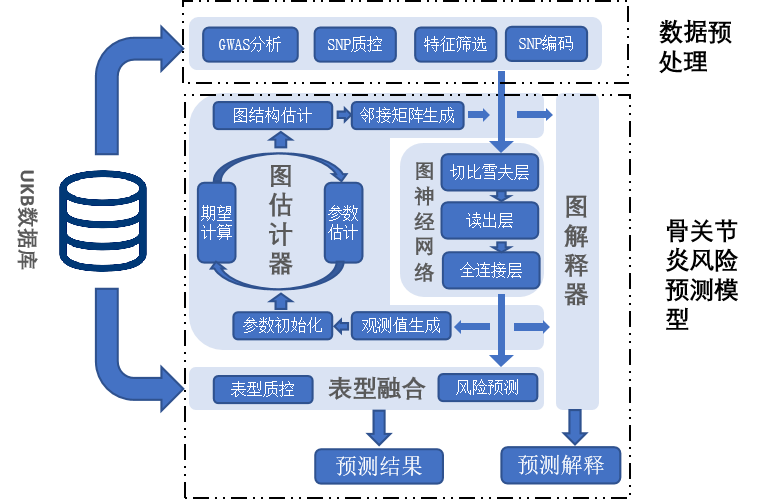
\includegraphics[width=\textwidth]{./figures/Chapter1/Routine.png}
	\caption{技术路线图} \label{fig:Routine}
\end{figure}